\begin{tikzpicture}
	\pgfplotsset{/tikz/font={\small}}
	\begin{axis}[
			xlabel={number of additional $8\times8$ incomplete transforms},
			%ylabel={overall ${\Vert\cdot\Vert}^2+\lambda{\Vert\cdot\Vert}_0$},
			grid=both,
			scale only axis,
			width=0.9\textwidth,
			height=0.6\textheight,
			ytick={60,70,...,100},
			y tick label style={
				/pgf/number format/.cd,
				fixed,
				fixed zerofill,
				precision=0,
				/tikz/.cd
			},
			%xmode=log,
			%log basis x={2},
			xtick={0, 1, 2, 4, 8, 16, 32},
			%xticklabels={0, 1, 2, 4, 8, 16, 32, 64},
			yticklabel=\pgfmathprintnumber{\tick}\,\%,
			xmin=0, xmax=32,
			ymin=60, ymax=100,
			%xmin=0.5, xmax=128,
			%ymin=29, ymax=32,
			%legend entries={DCT, DST, RDOT},
			%legend style={nodes=right},
			%legend pos= north east
		]

		\addplot[red, thick, mark=*,mark size=1pt] table {
		0		100
		1		92.2
		2		86
		4		81
		8		76.1
		16		70.4
		32		66.1
		};
	\end{axis}
\end{tikzpicture}
